
\documentclass{beamer}

\newtheorem{conjecture}{Conjecture}
 \newcommand{\bconj}[1]{\begin{conj}#1\end{conj}}
\newtheorem{mconj}{Metaconjecture}

\newtheorem{prop}{Proposition}
 \newcommand{\bprop}[1]{\begin{prop}#1\end{prop}}
\newtheorem{lem}{Lemma}
 \newcommand{\blem}[1]{\begin{lem}#1\end{lem}}


\newtheorem{guess}{Guess}
 \newcommand{\bguess}[1]{\begin{guess}#1\end{guess}}
%\newtheorem{corollary}{Corollary}



\usepackage{tikz,framed, amsrefs, amsthm}
\tikzstyle{every node}=[circle, draw, fill=black!50,
                        inner sep=0pt, minimum width=4pt]
\tikzstyle{lblvertex}=[fill=white, inner sep = 1pt, font=\small]
\tikzstyle{lblvertex2}=[fill=white, inner sep = 1pt, font=\tiny,circle, draw]
\tikzstyle{lblvertex3}=[fill=white, inner sep = 1pt, font=\tiny,circle, draw = black!25]
\tikzstyle{words} =[rectangle, draw=none, fill=none, black]
\newcommand{\bframe}[2]{\begin{frame}{#1}#2\end{frame}}
\newcommand{\bfig}[2]{\begin{figure}#1\caption{#2}\end{figure}}


\usetheme{CambridgeUS}
\setbeamertemplate{navigation symbols}{}
\usecolortheme[RGB={216,30,5}]{structure}
\AtBeginSection[] % "Beamer, do the following at the start of every section"
{
\begin{frame}<beamer>
\frametitle{Outline} % make a frame titled "Outline"
\tableofcontents[currentsection] % show TOC and highlight current section
\end{frame}
}

\title{Connected matchings in graphs}
\author{Chris Caragianis}
\institute[U of L]{ Department of Mathematics\\ University of Louisville\\ Louisville, KY 40292\\[1ex]
   \texttt{cjcara01@louisville.edu} }
\begin{document}

\bframe{}{\titlepage}

\bframe{}{\tableofcontents}

\section{Introduction: Connected matchings and Hadwiger's conjecture}

\subsection{Review of graph-theoretic concepts}

\bframe{Graphs, vertex coloring}{
	\begin{overprint} 
		\onslide<1>A (simple, undirected) graph is comprised of a collection of \textit{vertices}, some pairs of which are \textit{adjacent}.  A pair of adjacent vertices is called an \textit{edge}. \\
		\onslide<2-3>A (simple, undirected) graph is comprised of a collection of \textit{vertices}, some pairs of which are \textit{adjacent}.  A pair of adjacent vertices is called an \textit{edge}. \vskip 0.5 cm A proper vertex coloring is one in which adjacent vertices recieve different colors.
	\end{overprint}	
	\vskip 1 cm 
		\only<1-2>{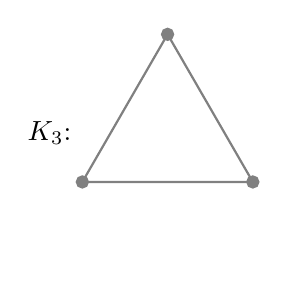
\begin{tikzpicture}[thick,scale=0.5]
\draw[gray] 
    {
		(180:3) node[words] {$K_3$:}
        (90:2.5) node {}  -- (210:2.5)
		(210:2.5) node {} -- (-30:2.5)
		(-30:2.5) node {} -- (90:2.5)
		(-90:3.5) node[words] {}
    };

\end{tikzpicture}
}\only<3>{\input{triangle_prop}} \qquad 
		\only<1-2>{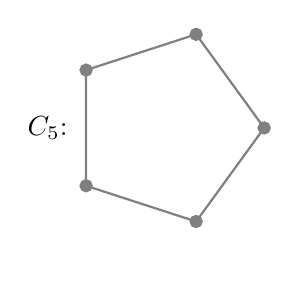
\begin{tikzpicture}[thick,scale=0.5]
\draw[gray] 
    {
		(180:3) node[words] {$C_5$:}
        (72:2.5) node {}  -- (144:2.5)
		(144:2.5) node {} -- (216:2.5)
		(216:2.5) node {} -- (288:2.5)
		(288:2.5) node {}  -- (0:2.5)
		(0:2.5) node {} -- (72:2.5)
		(-90:3.5) node[words] {}
    };
	
\end{tikzpicture}
}\only<3>{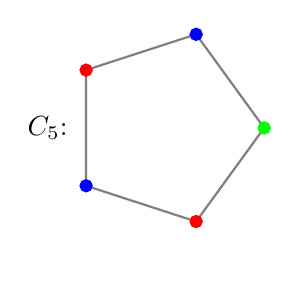
\begin{tikzpicture}[thick,scale=0.5]
\draw[gray] 
    {
		(180:3) node[words] {$C_5$:}
        (72:2.5) node[blue] {}  -- (144:2.5)
		(144:2.5) node[red] {} -- (216:2.5)
		(216:2.5) node[blue] {} -- (288:2.5)
		(288:2.5) node[red] {}  -- (0:2.5)
		(0:2.5) node[green] {} -- (72:2.5)
		(-90:3.5) node[words] {}
    };
	
\end{tikzpicture}
} \qquad 
		\only<1-2>{\begin{tikzpicture}[thick,scale=0.5]
\draw[gray] 
    {
		(180:3) node[words] {$G$:}
        (90:2.5) node {}  -- (0:0)
		(210:2.5) node {} -- (0:0)
		(-30:2.5) node {} -- (0:0)
		(0:0) node {}
		(-90:3.5) node[words] {}
    };

\end{tikzpicture}
}\only<3>{\begin{tikzpicture}[thick,scale=0.5]
\draw[gray] 
    {
		(180:3) node[words] {$G$:}
        (90:2.5) node[red] {}  -- (0:0)
		(210:2.5) node[red] {} -- (0:0)
		(-30:2.5) node[red] {} -- (0:0)
		(0:0) node[blue] {}
		(-90:3.5) node[words] {}
    };

\end{tikzpicture}
}}

\bframe{Clique number, independence number}{
	\begin{itemize}
		\item A \textit{clique} on $n$ vertices (also called a \textit{complete graph}) is a collection of $n$ vertices along with all possible edges.\pause  
		\item The \textit{clique number} of $G$, denoted $\omega(G)$, is the size of the largest clique in $G$.\pause  
		\item The \textit{independence number} of $G$, denoted $\alpha(G)$, is the size of the largest set of vertices from $G$ that induces no edges.\pause
	\end{itemize}
	\begin{center}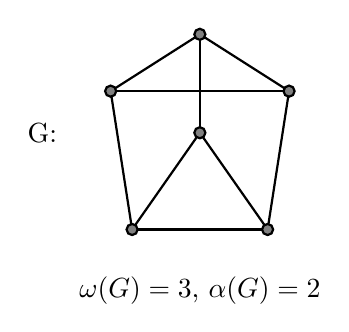
\begin{tikzpicture}[thick,scale=0.5]

	\coordinate (a) at (90:2.5);
	\coordinate (b) at (25:2.5); 
	\coordinate (c) at (0:0);
	\coordinate (d) at (155:2.5);
	\coordinate (e) at (-55:3);
	\coordinate (f) at (-125:3);

	\draw (a)--(b);
	%\draw (b)--(c);
	\draw (d)--(a);
	\draw (a)--(c);
	%\draw (c)--(d);
	\draw (b)--(e);
	\draw (e)--(c);
	\draw (d)--(f);
	\draw (f)--(c);
	\draw (d)--(b);
	\draw (e)--(f);
	%\draw (f) arc {-125:-33:3};
	
	\draw (a) node {};
	\draw (b) node {};
	\draw (c) node {};
	\draw (d) node {};
	\draw (e) node {};
	\draw (f) node {};
	\draw (-90:4) node[words] {$\omega(G) = 3$, $\alpha(G) = 2$};
	\draw (180:4) node[words] {G:};
\end{tikzpicture}
\end{center}}

\bframe{Chromatic number}{The \textit{chromatic number} of a graph $G$, denoted $\chi(G)$, is the minimum number of colors needed to properly color the vertices of $G$.
	\begin{overprint}	
		\onslide<1>\vskip 1 cm \input{triangle_prop} \qquad 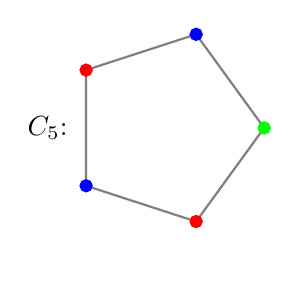
\begin{tikzpicture}[thick,scale=0.5]
\draw[gray] 
    {
		(180:3) node[words] {$C_5$:}
        (72:2.5) node[blue] {}  -- (144:2.5)
		(144:2.5) node[red] {} -- (216:2.5)
		(216:2.5) node[blue] {} -- (288:2.5)
		(288:2.5) node[red] {}  -- (0:2.5)
		(0:2.5) node[green] {} -- (72:2.5)
		(-90:3.5) node[words] {}
    };
	
\end{tikzpicture}
 \qquad \begin{tikzpicture}[thick,scale=0.5]
\draw[gray] 
    {
		(180:3) node[words] {$G$:}
        (90:2.5) node[red] {}  -- (0:0)
		(210:2.5) node[red] {} -- (0:0)
		(-30:2.5) node[red] {} -- (0:0)
		(0:0) node[blue] {}
		(-90:3.5) node[words] {}
    };

\end{tikzpicture}
\\
		\onslide<2>\vskip 1 cm \input{triangle_prop_chi} \qquad \input{c5_prop_chi} \qquad \input{claw_prop_chi}
	\end{overprint}}


\bframe{Perfect graphs}{
	Obviously, for any graph $G$, $\chi(G) \geq \omega(G)$, but the converse is not true.\pause\vskip 0.5 cm
	We say that a graph $G$ is \textit{perfect} if for every induced subgraph $H$ of $G$, the chromatic number is equal to the size of the largest complete subgraph of $H$.\pause

 	\vskip 1 cm \begin{theorem}[Strong perfect graph theorem (SPGT)]A graph $G$ is perfect if and only if for each $k >1$ it has neither a $C_{2k+1}$ nor its complement as an induced subgraph.\end{theorem}}

\bframe{Graph minors}{We say that a graph $G$ contains $H$ \textit{as a minor}, (denoted $G\geq H$), if $H$ is obtained from $G$ by successive vertex deletions and edge contractions.
	 }

\subsection{Hadwiger's conjecture}

\bframe{Hadwiger's conjecture}{
     It is widely believed, but is yet to be proved, that the size of the largest complete minor in a graph is an upper bound on the chromatic number. \pause
\vskip 0.5 cm Formally, let $\eta(G)$ be the largest $n$ for which $G \geq K_n$.\pause
 \vskip 1 cm \begin{conjecture}[Hadwiger, 1943] For all graphs $G$, \[\eta(G) \geq \chi(G)\] \end{conjecture} }

\bframe{Independence number and a weaker conjecture}{
	A special case that has received much attention is the class of graphs with independence number two.  \pause \vskip 0.5 cm
	Owing to the relation $n/\alpha(G) \geq \chi(G)$, the following conjecture is implied by Hadwiger's.\pause
 \begin{conjecture}\label{hc}
    For any graph $G$ on $n$ vertices with $\alpha(G) =2$, \[\eta(G) \geq \frac{n}{2}\]
 \end{conjecture}\pause
	Plummer, Stiebitz and Toft  show in \cite{MR2070161} that this is equivalent to Hadwiger's conjecture for graphs with independence number two.}

\subsection{Connected matchings}

\bframe{Connected matchings}{
	Connected matchings have played an important role in the study of this conjecture.\pause\vskip 0.5 cm
	 A \textit{connected matching} is a collection of disjoint edges such that each pair of edges has some edge between them.
	\begin{center}
	\begin{overprint}
		\onslide<3>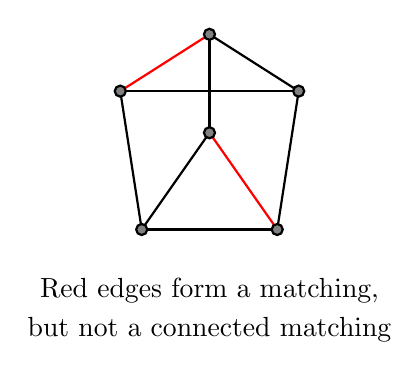
\begin{tikzpicture}[thick,scale=0.5]

	\coordinate (a) at (90:2.5);
	\coordinate (b) at (25:2.5); 
	\coordinate (c) at (0:0);
	\coordinate (d) at (155:2.5);
	\coordinate (e) at (-55:3);
	\coordinate (f) at (-125:3);

	\draw (a)--(b);
	%\draw (b)--(c);
	\draw[red] (d)--(a);
	\draw (a)--(c);
	%\draw (c)--(d);
	\draw (b)--(e);
	\draw[red] (e)--(c);
	\draw (d)--(f);
	\draw (f)--(c);
	\draw (d)--(b);
	\draw (e)--(f);
	%\draw (f) arc {-125:-33:3};
	
	\draw (a) node {};
	\draw (b) node {};
	\draw (c) node {};
	\draw (d) node {};
	\draw (e) node {};
	\draw (f) node {};
	\draw (-90:4) node[words] {Red edges form a matching,};
	\draw (-90:5) node[words] {but not a connected matching};
\end{tikzpicture}
\\
		\onslide<4-> 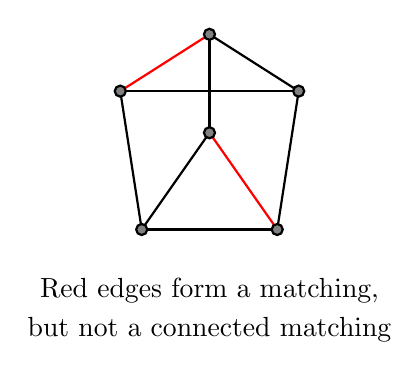
\begin{tikzpicture}[thick,scale=0.5]

	\coordinate (a) at (90:2.5);
	\coordinate (b) at (25:2.5); 
	\coordinate (c) at (0:0);
	\coordinate (d) at (155:2.5);
	\coordinate (e) at (-55:3);
	\coordinate (f) at (-125:3);

	\draw (a)--(b);
	%\draw (b)--(c);
	\draw[red] (d)--(a);
	\draw (a)--(c);
	%\draw (c)--(d);
	\draw (b)--(e);
	\draw[red] (e)--(c);
	\draw (d)--(f);
	\draw (f)--(c);
	\draw (d)--(b);
	\draw (e)--(f);
	%\draw (f) arc {-125:-33:3};
	
	\draw (a) node {};
	\draw (b) node {};
	\draw (c) node {};
	\draw (d) node {};
	\draw (e) node {};
	\draw (f) node {};
	\draw (-90:4) node[words] {Red edges form a matching,};
	\draw (-90:5) node[words] {but not a connected matching};
\end{tikzpicture}
\qquad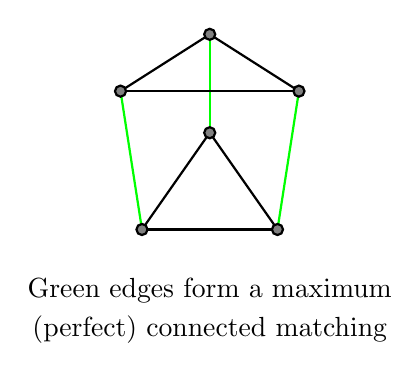
\begin{tikzpicture}[thick,scale=0.5]

	\coordinate (a) at (90:2.5);
	\coordinate (b) at (25:2.5); 
	\coordinate (c) at (0:0);
	\coordinate (d) at (155:2.5);
	\coordinate (e) at (-55:3);
	\coordinate (f) at (-125:3);

	\draw (a)--(b);
	%\draw (b)--(c);
	\draw (d)--(a);
	\draw[green] (a)--(c);
	%\draw (c)--(d);
	\draw[green] (b)--(e);
	\draw (e)--(c);
	\draw[green] (d)--(f);
	\draw (f)--(c);
	\draw (d)--(b);
	\draw (e)--(f);
	%\draw (f) arc {-125:-33:3};
	
	\draw (a) node {};
	\draw (b) node {};
	\draw (c) node {};
	\draw (d) node {};
	\draw (e) node {};
	\draw (f) node {};
	\draw (-90:4) node[words] {Green edges form a maximum};
	\draw (-90:5) node[words] {(perfect) connected matching};
\end{tikzpicture}

	\end{overprint}
	\end{center}
	\uncover<5->{Note that a connected matching of $t$ edges contains $K_{t}$ as a minor.}}

\bframe{An extremal conjecture for connected matchings}{
  Gy\'arf\'as, F\"uredi and Simonyi observe this and conjecture \pause 
 	\begin{conjecture}[\cite{FGS}]
  		There exists an absolute constant $c$ so that any graph $G$ with $\alpha(G) =2$ and at least $ct$ vertices has a connected matching of at least $t$ edges.
 	\end{conjecture}\vskip 0.5 cm\pause
 	If true, this would establish that when $\alpha(G) = 2$, $\eta(G) > n/3$. This would improve the best known bound of $1/(2\alpha-1)$ shown by Duchet and Meyniel \cite{MR671905}.  \vskip 0.5 cm \pause Gy\'arf\'as et al. further conjecture that $c = 4$ and prove this for $t \leq 17$.}

\section{Connected matchings and optimization}

\bframe{Clique problems}{
	Any system of nodes with a symmetric relation can be modeled with an undirected graph.\pause\vskip 0.5cm
	If we wish to find the largest possible set of mutually related nodes in the system, then we are presented with a maximum clique problem (MAX CLIQUE).\pause\vskip 0.5cm
	}

\bframe{Clique minors}{
	We can generalize the clique problem to the clique-\textit{minor} problem:  \pause that is, find the largest $t$ for which $G \geq K_t$.\pause\vskip 0.5 cm
	 A $t$-clique minor is composed of $t$ connected subgraphs each of which sends an edge into all others.  \pause  Upon contracting the edges of each connected subgraphs to a single vertex, one obtains a clique on $t$ vertices. \pause\vskip 0.5 cm
	We can illustrate the type of optimization performed by the clique and the clique minor problem with a hypothetical scenario.}

\bframe{Clique and clique-minor optimization}{
	Suppose there are $n$ people at a party.  \uncover<3->{We construct a graph on $n$ vertices representing partygoers with an edge between $u$ and $v$ if the corresponding partygoers are friendly.}\pause\vskip 0.5 cm 
	\begin{center}	
	\begin{overprint}[6 cm]
		\onslide<2-3>\begin{tikzpicture}[thick,scale=0.5]

	\coordinate (a1) at (22:5);
	\coordinate (a2) at (44.5:5);
	\coordinate (a3) at (67:5);
	\coordinate (a4) at (89.5:5);
	\coordinate (a5) at (112:5);
	\coordinate (a6) at (134.5:5);
	\coordinate (a7) at (157:5);
	\coordinate (a8) at (179.5:5);
	\coordinate (a9) at (202:5);
	\coordinate (a10) at (224.5:5);
	\coordinate (a11) at (247:5);
	\coordinate (a12) at (269.5:5);
	\coordinate (a13) at (292:5);
	\coordinate (a14) at (314.5:5);
	\coordinate (a15) at (337:5);
	\coordinate (a16) at (359.5:5);

	\draw (a1) node[lblvertex2] {a};
	\draw (a2) node[lblvertex2] {b};
	\draw (a3) node[lblvertex2] {c};
	\draw (a4) node[lblvertex2] {d};
	\draw (a5) node[lblvertex2] {e};
	\draw (a6) node[lblvertex2] {f};
	\draw (a7) node[lblvertex2] {g};
	\draw (a8) node[lblvertex2] {h};
	\draw (a9) node[lblvertex2] {i};
	\draw (a10) node[lblvertex2] {j};
	\draw (a11) node[lblvertex2] {k};
	\draw (a12) node[lblvertex2] {l};
	\draw (a13) node[lblvertex2] {m};
	\draw (a14) node[lblvertex2] {n};
	\draw (a15) node[lblvertex2] {o};
	\draw (a16) node[lblvertex2] {p};
\end{tikzpicture}

		\onslide<4>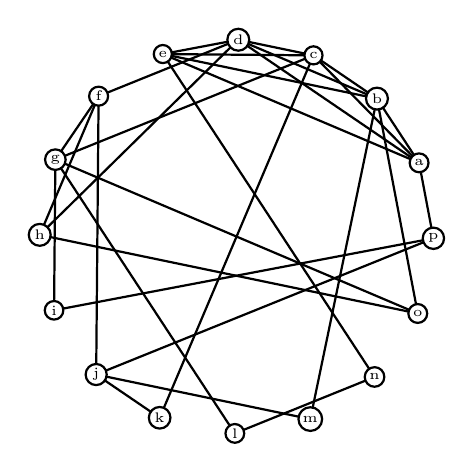
\begin{tikzpicture}[thick,scale=0.5]

	\coordinate (a1) at (22:5);
	\coordinate (a2) at (44.5:5);
	\coordinate (a3) at (67:5);
	\coordinate (a4) at (89.5:5);
	\coordinate (a5) at (112:5);
	\coordinate (a6) at (134.5:5);
	\coordinate (a7) at (157:5);
	\coordinate (a8) at (179.5:5);
	\coordinate (a9) at (202:5);
	\coordinate (a10) at (224.5:5);
	\coordinate (a11) at (247:5);
	\coordinate (a12) at (269.5:5);
	\coordinate (a13) at (292:5);
	\coordinate (a14) at (314.5:5);
	\coordinate (a15) at (337:5);
	\coordinate (a16) at (359.5:5);

	% the K_5
	\draw (a1) -- (a2);
	\draw (a1) -- (a3);
	\draw (a1) -- (a4);
	\draw (a1) -- (a5);
	\draw (a2) -- (a3);
	\draw (a2) -- (a4);
	\draw (a2) -- (a5);
	\draw (a3) -- (a4);
	\draw (a3) -- (a5);
	\draw (a4) -- (a5);

	% the connmatch
	\draw (a1) -- (a16);
	\draw (a2) -- (a13);
	\draw (a3) -- (a11);	
	\draw (a6) -- (a10); %new	
	\draw (a8) -- (a4);
	\draw (a5) -- (a14);
	
	% connect it up
	\draw (a6) -- (a4); 
	\draw (a6) -- (a8);
	\draw (a10) -- (a11);
	\draw (a10) -- (a13);
	\draw (a10) -- (a16);

	% the K_{1,3}
	\draw (a7) -- (a9);
	\draw (a7) -- (a15);
	\draw (a7) -- (a12);
	
	% connect THAT up
	\draw (a7) -- (a6);
	\draw (a7) -- (a3);
	\draw (a9) -- (a16);
	\draw (a15) -- (a2);
	\draw (a12) -- (a14);
	\draw (a15) -- (a8);
	% the nodes
	\draw (a1) node[lblvertex2] {a};
	\draw (a2) node[lblvertex2] {b};
	\draw (a3) node[lblvertex2] {c};
	\draw (a4) node[lblvertex2] {d};
	\draw (a5) node[lblvertex2] {e};
	\draw (a6) node[lblvertex2] {f};
	\draw (a7) node[lblvertex2] {g};
	\draw (a8) node[lblvertex2] {h};
	\draw (a9) node[lblvertex2] {i};
	\draw (a10) node[lblvertex2] {j};
	\draw (a11) node[lblvertex2] {k};
	\draw (a12) node[lblvertex2] {l};
	\draw (a13) node[lblvertex2] {m};
	\draw (a14) node[lblvertex2] {n};
	\draw (a15) node[lblvertex2] {o};
	\draw (a16) node[lblvertex2] {p};
	
\end{tikzpicture}

	\end{overprint}
	\end{center}
}
\bframe{Clique and clique-minor optimization}{
	On this graph, the clique problem looks for the largest collection of mutually freindly partygoers.\vskip 0.5 cm
	\begin{center}	
	\begin{overprint}[6 cm]
		\onslide<1>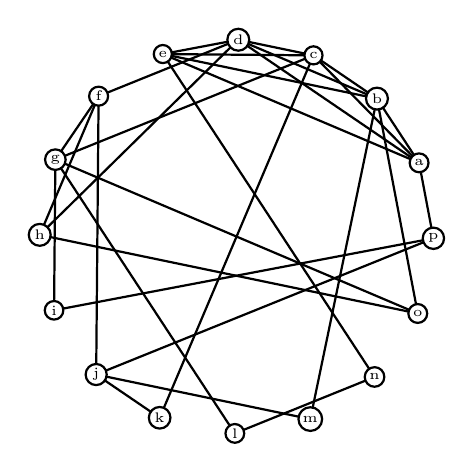
\begin{tikzpicture}[thick,scale=0.5]

	\coordinate (a1) at (22:5);
	\coordinate (a2) at (44.5:5);
	\coordinate (a3) at (67:5);
	\coordinate (a4) at (89.5:5);
	\coordinate (a5) at (112:5);
	\coordinate (a6) at (134.5:5);
	\coordinate (a7) at (157:5);
	\coordinate (a8) at (179.5:5);
	\coordinate (a9) at (202:5);
	\coordinate (a10) at (224.5:5);
	\coordinate (a11) at (247:5);
	\coordinate (a12) at (269.5:5);
	\coordinate (a13) at (292:5);
	\coordinate (a14) at (314.5:5);
	\coordinate (a15) at (337:5);
	\coordinate (a16) at (359.5:5);

	% the K_5
	\draw (a1) -- (a2);
	\draw (a1) -- (a3);
	\draw (a1) -- (a4);
	\draw (a1) -- (a5);
	\draw (a2) -- (a3);
	\draw (a2) -- (a4);
	\draw (a2) -- (a5);
	\draw (a3) -- (a4);
	\draw (a3) -- (a5);
	\draw (a4) -- (a5);

	% the connmatch
	\draw (a1) -- (a16);
	\draw (a2) -- (a13);
	\draw (a3) -- (a11);	
	\draw (a6) -- (a10); %new	
	\draw (a8) -- (a4);
	\draw (a5) -- (a14);
	
	% connect it up
	\draw (a6) -- (a4); 
	\draw (a6) -- (a8);
	\draw (a10) -- (a11);
	\draw (a10) -- (a13);
	\draw (a10) -- (a16);

	% the K_{1,3}
	\draw (a7) -- (a9);
	\draw (a7) -- (a15);
	\draw (a7) -- (a12);
	
	% connect THAT up
	\draw (a7) -- (a6);
	\draw (a7) -- (a3);
	\draw (a9) -- (a16);
	\draw (a15) -- (a2);
	\draw (a12) -- (a14);
	\draw (a15) -- (a8);
	% the nodes
	\draw (a1) node[lblvertex2] {a};
	\draw (a2) node[lblvertex2] {b};
	\draw (a3) node[lblvertex2] {c};
	\draw (a4) node[lblvertex2] {d};
	\draw (a5) node[lblvertex2] {e};
	\draw (a6) node[lblvertex2] {f};
	\draw (a7) node[lblvertex2] {g};
	\draw (a8) node[lblvertex2] {h};
	\draw (a9) node[lblvertex2] {i};
	\draw (a10) node[lblvertex2] {j};
	\draw (a11) node[lblvertex2] {k};
	\draw (a12) node[lblvertex2] {l};
	\draw (a13) node[lblvertex2] {m};
	\draw (a14) node[lblvertex2] {n};
	\draw (a15) node[lblvertex2] {o};
	\draw (a16) node[lblvertex2] {p};
	
\end{tikzpicture}

		\onslide<2>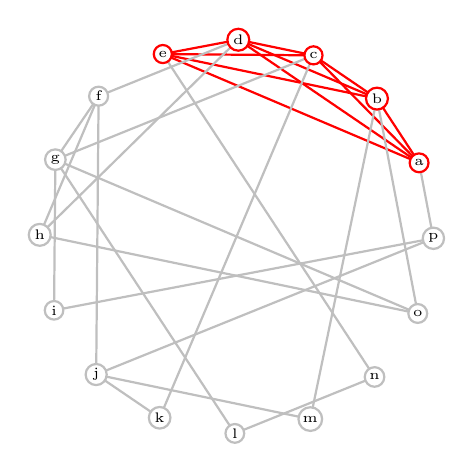
\begin{tikzpicture}[thick,scale=0.5]

	\coordinate (a1) at (22:5);
	\coordinate (a2) at (44.5:5);
	\coordinate (a3) at (67:5);
	\coordinate (a4) at (89.5:5);
	\coordinate (a5) at (112:5);
	\coordinate (a6) at (134.5:5);
	\coordinate (a7) at (157:5);
	\coordinate (a8) at (179.5:5);
	\coordinate (a9) at (202:5);
	\coordinate (a10) at (224.5:5);
	\coordinate (a11) at (247:5);
	\coordinate (a12) at (269.5:5);
	\coordinate (a13) at (292:5);
	\coordinate (a14) at (314.5:5);
	\coordinate (a15) at (337:5);
	\coordinate (a16) at (359.5:5);

	% the K_5
	\draw (a1)[red] -- (a2);
	\draw (a1)[red] -- (a3);
	\draw (a1)[red] -- (a4);
	\draw (a1)[red] -- (a5);
	\draw (a2)[red] -- (a3);
	\draw (a2)[red] -- (a4);
	\draw (a2)[red] -- (a5);
	\draw (a3)[red] -- (a4);
	\draw (a3)[red] -- (a5);
	\draw (a4)[red] -- (a5);

	% the connmatch
	\draw (a1)[black!25] -- (a16);
	\draw (a2)[black!25] -- (a13);
	\draw (a3)[black!25] -- (a11);	
	\draw (a6)[black!25] -- (a10); %new	
	\draw (a8)[black!25] -- (a4);
	\draw (a5)[black!25] -- (a14);
	
	% connect it up
	\draw (a6)[black!25] -- (a4); 
	\draw (a6)[black!25] -- (a8);
	\draw (a10)[black!25] -- (a11);
	\draw (a10)[black!25] -- (a13);
	\draw (a10)[black!25] -- (a16);

	% the K_{1,3}
	\draw (a7)[black!25] -- (a9);
	\draw (a7)[black!25] -- (a15);
	\draw (a7)[black!25] -- (a12);
	
	% connect THAT up
	\draw (a7)[black!25] -- (a6);
	\draw (a7)[black!25] -- (a3);
	\draw (a9)[black!25] -- (a16);
	\draw (a15)[black!25] -- (a2);
	\draw (a12)[black!25] -- (a14);
	\draw (a15)[black!25] -- (a8);

	% the nodes
	\draw (a1) node[lblvertex3, draw = red] {a};
	\draw (a2) node[lblvertex3, draw = red] {b};
	\draw (a3) node[lblvertex3, draw = red] {c};
	\draw (a4) node[lblvertex3, draw = red] {d};
	\draw (a5) node[lblvertex3, draw = red] {e};
	\draw (a6) node[lblvertex3] {f};
	\draw (a7) node[lblvertex3] {g};
	\draw (a8) node[lblvertex3] {h};
	\draw (a9) node[lblvertex3] {i};
	\draw (a10) node[lblvertex3] {j};
	\draw (a11) node[lblvertex3] {k};
	\draw (a12) node[lblvertex3] {l};
	\draw (a13) node[lblvertex3] {m};
	\draw (a14) node[lblvertex3] {n};
	\draw (a15) node[lblvertex3] {o};
	\draw (a16) node[lblvertex3] {p};

	
\end{tikzpicture}

	\end{overprint}
	\end{center}
}

\bframe{}{	
	Now suppose we allow partygoers to form teams in which each team member introduces the team to all partygoers with whom she is friendly. \vskip 0.5 cm
 \uncover<2->{The clique minor problem on this graph asks for the largest number of mutually friendly teams that can be formed.}
	\begin{center}	
	\begin{overprint}[6 cm]
		\onslide<1-2>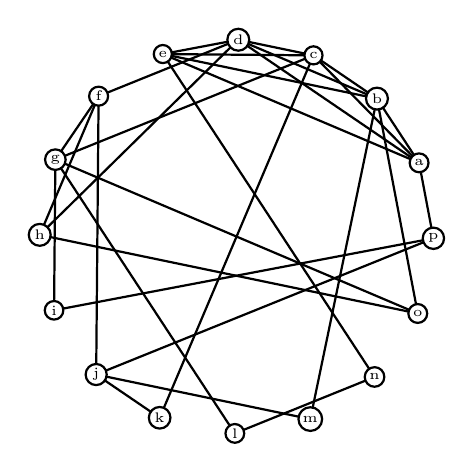
\begin{tikzpicture}[thick,scale=0.5]

	\coordinate (a1) at (22:5);
	\coordinate (a2) at (44.5:5);
	\coordinate (a3) at (67:5);
	\coordinate (a4) at (89.5:5);
	\coordinate (a5) at (112:5);
	\coordinate (a6) at (134.5:5);
	\coordinate (a7) at (157:5);
	\coordinate (a8) at (179.5:5);
	\coordinate (a9) at (202:5);
	\coordinate (a10) at (224.5:5);
	\coordinate (a11) at (247:5);
	\coordinate (a12) at (269.5:5);
	\coordinate (a13) at (292:5);
	\coordinate (a14) at (314.5:5);
	\coordinate (a15) at (337:5);
	\coordinate (a16) at (359.5:5);

	% the K_5
	\draw (a1) -- (a2);
	\draw (a1) -- (a3);
	\draw (a1) -- (a4);
	\draw (a1) -- (a5);
	\draw (a2) -- (a3);
	\draw (a2) -- (a4);
	\draw (a2) -- (a5);
	\draw (a3) -- (a4);
	\draw (a3) -- (a5);
	\draw (a4) -- (a5);

	% the connmatch
	\draw (a1) -- (a16);
	\draw (a2) -- (a13);
	\draw (a3) -- (a11);	
	\draw (a6) -- (a10); %new	
	\draw (a8) -- (a4);
	\draw (a5) -- (a14);
	
	% connect it up
	\draw (a6) -- (a4); 
	\draw (a6) -- (a8);
	\draw (a10) -- (a11);
	\draw (a10) -- (a13);
	\draw (a10) -- (a16);

	% the K_{1,3}
	\draw (a7) -- (a9);
	\draw (a7) -- (a15);
	\draw (a7) -- (a12);
	
	% connect THAT up
	\draw (a7) -- (a6);
	\draw (a7) -- (a3);
	\draw (a9) -- (a16);
	\draw (a15) -- (a2);
	\draw (a12) -- (a14);
	\draw (a15) -- (a8);
	% the nodes
	\draw (a1) node[lblvertex2] {a};
	\draw (a2) node[lblvertex2] {b};
	\draw (a3) node[lblvertex2] {c};
	\draw (a4) node[lblvertex2] {d};
	\draw (a5) node[lblvertex2] {e};
	\draw (a6) node[lblvertex2] {f};
	\draw (a7) node[lblvertex2] {g};
	\draw (a8) node[lblvertex2] {h};
	\draw (a9) node[lblvertex2] {i};
	\draw (a10) node[lblvertex2] {j};
	\draw (a11) node[lblvertex2] {k};
	\draw (a12) node[lblvertex2] {l};
	\draw (a13) node[lblvertex2] {m};
	\draw (a14) node[lblvertex2] {n};
	\draw (a15) node[lblvertex2] {o};
	\draw (a16) node[lblvertex2] {p};
	
\end{tikzpicture}

		\onslide<3>\input{party4}
	\end{overprint}
	\end{center}}

\bframe{Connected matching as a special case of clique minor}{
	A connected matching is a special case of a clique minor in which each ``team'' has exactly two members.    \vskip 0.25 cm
	\uncover<2->{The maximum connected matching problem asks for the maximum number of \textit{pairs} that can be formed so that all pairs are friendly.}
	\begin{center}	
	\begin{overprint}[6 cm]
		\onslide<1-2>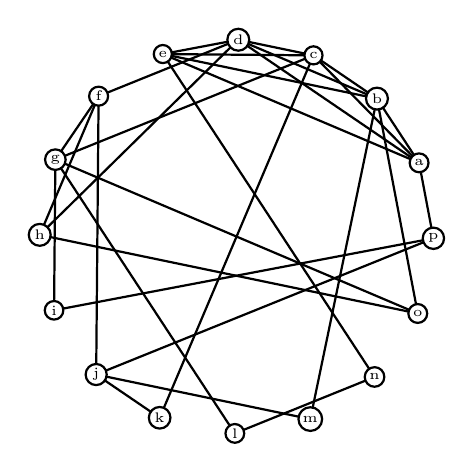
\begin{tikzpicture}[thick,scale=0.5]

	\coordinate (a1) at (22:5);
	\coordinate (a2) at (44.5:5);
	\coordinate (a3) at (67:5);
	\coordinate (a4) at (89.5:5);
	\coordinate (a5) at (112:5);
	\coordinate (a6) at (134.5:5);
	\coordinate (a7) at (157:5);
	\coordinate (a8) at (179.5:5);
	\coordinate (a9) at (202:5);
	\coordinate (a10) at (224.5:5);
	\coordinate (a11) at (247:5);
	\coordinate (a12) at (269.5:5);
	\coordinate (a13) at (292:5);
	\coordinate (a14) at (314.5:5);
	\coordinate (a15) at (337:5);
	\coordinate (a16) at (359.5:5);

	% the K_5
	\draw (a1) -- (a2);
	\draw (a1) -- (a3);
	\draw (a1) -- (a4);
	\draw (a1) -- (a5);
	\draw (a2) -- (a3);
	\draw (a2) -- (a4);
	\draw (a2) -- (a5);
	\draw (a3) -- (a4);
	\draw (a3) -- (a5);
	\draw (a4) -- (a5);

	% the connmatch
	\draw (a1) -- (a16);
	\draw (a2) -- (a13);
	\draw (a3) -- (a11);	
	\draw (a6) -- (a10); %new	
	\draw (a8) -- (a4);
	\draw (a5) -- (a14);
	
	% connect it up
	\draw (a6) -- (a4); 
	\draw (a6) -- (a8);
	\draw (a10) -- (a11);
	\draw (a10) -- (a13);
	\draw (a10) -- (a16);

	% the K_{1,3}
	\draw (a7) -- (a9);
	\draw (a7) -- (a15);
	\draw (a7) -- (a12);
	
	% connect THAT up
	\draw (a7) -- (a6);
	\draw (a7) -- (a3);
	\draw (a9) -- (a16);
	\draw (a15) -- (a2);
	\draw (a12) -- (a14);
	\draw (a15) -- (a8);
	% the nodes
	\draw (a1) node[lblvertex2] {a};
	\draw (a2) node[lblvertex2] {b};
	\draw (a3) node[lblvertex2] {c};
	\draw (a4) node[lblvertex2] {d};
	\draw (a5) node[lblvertex2] {e};
	\draw (a6) node[lblvertex2] {f};
	\draw (a7) node[lblvertex2] {g};
	\draw (a8) node[lblvertex2] {h};
	\draw (a9) node[lblvertex2] {i};
	\draw (a10) node[lblvertex2] {j};
	\draw (a11) node[lblvertex2] {k};
	\draw (a12) node[lblvertex2] {l};
	\draw (a13) node[lblvertex2] {m};
	\draw (a14) node[lblvertex2] {n};
	\draw (a15) node[lblvertex2] {o};
	\draw (a16) node[lblvertex2] {p};
	
\end{tikzpicture}

		\onslide<3>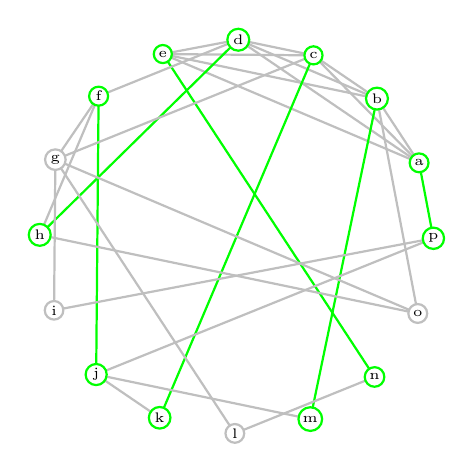
\begin{tikzpicture}[thick,scale=0.5]

	\coordinate (a1) at (22:5);
	\coordinate (a2) at (44.5:5);
	\coordinate (a3) at (67:5);
	\coordinate (a4) at (89.5:5);
	\coordinate (a5) at (112:5);
	\coordinate (a6) at (134.5:5);
	\coordinate (a7) at (157:5);
	\coordinate (a8) at (179.5:5);
	\coordinate (a9) at (202:5);
	\coordinate (a10) at (224.5:5);
	\coordinate (a11) at (247:5);
	\coordinate (a12) at (269.5:5);
	\coordinate (a13) at (292:5);
	\coordinate (a14) at (314.5:5);
	\coordinate (a15) at (337:5);
	\coordinate (a16) at (359.5:5);

	% the K_5
	\draw (a1)[black!25] -- (a2);
	\draw (a1)[black!25] -- (a3);
	\draw (a1)[black!25] -- (a4);
	\draw (a1)[black!25] -- (a5);
	\draw (a2)[black!25] -- (a3);
	\draw (a2)[black!25] -- (a4);
	\draw (a2)[black!25] -- (a5);
	\draw (a3)[black!25] -- (a4);
	\draw (a3)[black!25] -- (a5);
	\draw (a4)[black!25] -- (a5);

	% the connmatch
	\draw (a1)[green] -- (a16);
	\draw (a2)[green] -- (a13);
	\draw (a3)[green] -- (a11);	
	\draw (a6)[green] -- (a10); %new	
	\draw (a8)[green] -- (a4);
	\draw (a5)[green] -- (a14);
	
	% connect it up
	\draw (a6)[black!25] -- (a4); 
	\draw (a6)[black!25] -- (a8);
	\draw (a10)[black!25] -- (a11);
	\draw (a10)[black!25] -- (a13);
	\draw (a10)[black!25] -- (a16);

	% the K_{1,3}
	\draw (a7)[black!25] -- (a9);
	\draw (a7)[black!25] -- (a15);
	\draw (a7)[black!25] -- (a12);
	
	% connect THAT up
	\draw (a7)[black!25] -- (a6);
	\draw (a7)[black!25] -- (a3);
	\draw (a9)[black!25] -- (a16);
	\draw (a15)[black!25] -- (a2);
	\draw (a12)[black!25] -- (a14);
	\draw (a15)[black!25] -- (a8);

	% the nodes
	\draw (a1) node[lblvertex3, draw = green] {a};
	\draw (a2) node[lblvertex3, draw = green] {b};
	\draw (a3) node[lblvertex3, draw = green] {c};
	\draw (a4) node[lblvertex3, draw = green] {d};
	\draw (a5) node[lblvertex3, draw = green] {e};
	\draw (a6) node[lblvertex3, draw = green] {f};
	\draw (a7) node[lblvertex3] {g};
	\draw (a8) node[lblvertex3, draw = green] {h};
	\draw (a9) node[lblvertex3] {i};
	\draw (a10) node[lblvertex3, draw = green] {j};
	\draw (a11) node[lblvertex3, draw = green] {k};
	\draw (a12) node[lblvertex3] {l};
	\draw (a13) node[lblvertex3, draw = green] {m};
	\draw (a14) node[lblvertex3, draw = green] {n};
	\draw (a15) node[lblvertex3] {o};
	\draw (a16) node[lblvertex3, draw = green] {p};

	
\end{tikzpicture}

	\end{overprint}
	\end{center}}

\section{Maximum Connected Matching}

\bframe{Two computational problems}{
	Given an input graph we would like to be able to find a maximum connected matching.\pause
 	\begin{framed}
  		Maximum Connected Matching (MCM)
  		\vskip 0.25 cm Input: Graph $G$
  		\newline Output: Maximum connected matching of $G$
 	\end{framed}\pause
	We also may be interested in the largest connected portion of a given matching in $G$\pause
 	\begin{framed}
  		Maximum Connected Portion (MCP)
  		\vskip 0.25 cm Input: A matching $M$ from a graph $G$
  		\newline Output: Maximum connected portion of $M$
 	\end{framed}}

\bframe{Complexity results}{
	Both MCM and MCP are NP-hard in general.\pause\vskip 0.5 cm
	We will show a reduction of MCP to MAX CLIQUE, further demonstrating that it is difficult to approximate.  Naturally, this extends to MCM. \pause\vskip 0.5 cm
	 Katie Cameron has shown that MCM remains NP-hard for bipartite graphs \cite{MR2163948}.\pause\vskip 0.5 cm
	 However, the problem is trivial for graphs with girth larger than 6 (hence, trees).\pause\vskip 0.5 cm
	Cameron also shows that MCM is polytime solvable on the class of \textit{chordal graphs}.}
	 
\bframe{Positive results and conjectures}{
	
	We will show that MCP is polytime solvable for a polytime-recognizable class of graphs with independence number 2. \pause\vskip 0.5 cm
	We will also offer the following conjecture:\pause
	\begin{conjecture}
		MCM is polytime solvable on the class of graphs with independence number 2.  
	\end{conjecture}\pause
	One approach to this conjecture will be to consider the following problem:\pause
	\begin{problem}
		Determine conditions for $G$ under which there is a polynomial reduction of MCM to MCP.
	\end{problem}\pause
}

\section{Proximity Partitions}

\subsection{Basic facts and definitions}

\bframe{Definition}{
	Given a graph $G$ on $n$ vertices, we define the \textit{proximity $k$-partition} $\mathcal{P} = \{P_1, P_2, \ldots, P_k\}$ of the edges of $K_n$ induced by $G$ as follows.\pause\vskip 0.5 cm

	For all $u,v \in V(G)$, $i < k$
 	\begin{enumerate}
  		\item $uv \in P_i$ if and only if $d_G(u,v) = i$\pause
  		\item $uv \in P_k$ if and only if $d_G(u,v) \geq k$\pause
 	\end{enumerate}
	\vskip 0.5 cm
	\begin{center}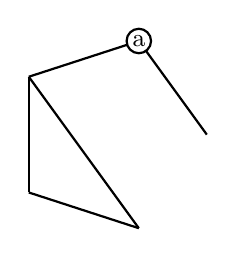
\begin{tikzpicture}[thick,scale=0.5]

	\coordinate (a1) at (72:2.5);
	\coordinate (a2) at (144:2.5); 
	\coordinate (a3) at (216:2.5);
	\coordinate (a4) at (288:2.5);
	\coordinate (a5) at (0:2.5);

	\draw (a5)--(a1);
	\draw (a1)--(a2);
	\draw (a2)--(a3);
	\draw (a2)--(a4);
	\draw (a3)--(a4);

	\draw (a1) node[lblvertex] {a};  
	
\end{tikzpicture}
\pause\quad 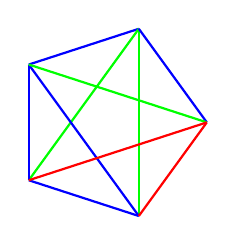
\begin{tikzpicture}[thick,scale=0.5]

	\coordinate (a1) at (72:2.5);
	\coordinate (a2) at (144:2.5); 
	\coordinate (a3) at (216:2.5);
	\coordinate (a4) at (288:2.5);
	\coordinate (a5) at (0:2.5);
	
	\draw[blue] (a1)--(a2);	
	\draw[green,] (a1)-- (a3);
	\draw[green] (a1)--(a4);
	\draw[blue] (a1)--(a5);
	\draw[blue] (a2)--(a3);	
	\draw[blue] (a2)--(a4);	
	\draw[green] (a2)--(a5);
	\draw[blue] (a3)--(a4);
	\draw[red] (a3)--(a5);
	\draw[red] (a4)--(a5);
	
	
\end{tikzpicture}
\end{center}}

\bframe{Proximity colorings}{
	We will be primarily interested in proximity 3-partitions, and for brevity will refer to these as \textit{proximity colorings}\pause\vskip 0.5cm
	As in the previous example, the distance 1 set will be ``blue'', the distance 2 set will be ``green'', and the distance 3 or greater set will be ``red''.\pause\vskip 0.5 cm
	We will also refer to the edges of a single color, green for instance, as the ``green graph of $G$''.}

\subsection{Connected matchings and proximity 3-coloring}

\bframe{Line graphs}{
	Recall the definition of a line graph.\pause\vskip 0.5 cm

	For any graph $G$, the \textit{line graph} of $G$, denoted $L(G)$, is the graph with vertex set equal to the edge set of $G$, with edges between vertices corresponding to incident edges in $G$.\pause\vskip 0.5 cm

	\begin{center}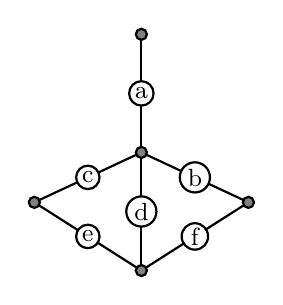
\begin{tikzpicture}[thick,scale=0.5]

	\coordinate (a1) at (90:3);
	\coordinate (a2) at (-25:3); 
	\coordinate (a3) at (-155:3);
	\coordinate (a4) at (-90:3);
	\coordinate (a5) at (0:0);

	\draw (a5)-- node [lblvertex] {a}(a1);
	\draw (a5)-- node [lblvertex] {b}(a2);
	\draw (a5)-- node [lblvertex] {c}(a3);
	\draw (a5)-- node [lblvertex] {d}(a4);
	\draw (a3)-- node [lblvertex] {e}(a4);
	\draw (a2)-- node [lblvertex] {f}(a4);

	\draw (a1) node {};
	\draw (a2) node {};
	\draw (a3) node {};
	\draw (a4) node {};
	\draw (a5) node {};
	%\draw (a1) node[lblvertex] {a};
	%\draw (a2) node[lblvertex] {b};  
	
\end{tikzpicture}
\pause\quad 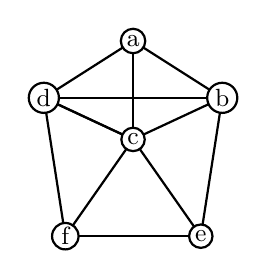
\begin{tikzpicture}[thick,scale=0.5]

	\coordinate (a) at (90:2.5);
	\coordinate (b) at (25:2.5); 
	\coordinate (c) at (0:0);
	\coordinate (d) at (155:2.5);
	\coordinate (e) at (-55:3);
	\coordinate (f) at (-125:3);

	\draw (a)--(b);
	\draw (b)--(c);
	\draw (c)--(d);
	\draw (d)--(a);
	\draw (a)--(c);
	\draw (c)--(d);
	\draw (b)--(e);
	\draw (e)--(c);
	\draw (d)--(f);
	\draw (f)--(c);
	\draw (d)--(b);
	\draw (e)--(f);
	%\draw (f) arc {-125:-33:3};
	
	\draw (a) node [lblvertex]{a};
	\draw (b) node [lblvertex]{b};
	\draw (c) node [lblvertex]{c};
	\draw (d) node [lblvertex]{d};
	\draw (e) node [lblvertex]{e};
	\draw (f) node [lblvertex]{f};
\end{tikzpicture}
\end{center}}
\bframe{Connected matching as a clique problem}{
	In the proximity coloring induced by $L(G)$
	\begin{itemize} 
		\uncover<2->{\item Blue edges correspond to a pair of incident edges in $G$} 
	 	\uncover<4->{\item Green edges correspond to a pair of disjoint edges in $G$ with some edge between them,} 
		\uncover<6->{\item Red edges correspond to disjoint and disconnected edges.}
	\end{itemize}
	\begin{center}
		\uncover<3->{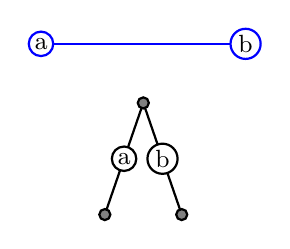
\begin{tikzpicture}[thick,scale=0.5]

	\coordinate (a0) at (0:0);
	\coordinate (a1) at (180:1);
	\coordinate (a3) at (-109:3);
	\coordinate (a2) at (0:1);
	\coordinate (a4) at (-71:3);
	\coordinate (b1) at (150:3);
	\coordinate (b2) at (30:3);

	\draw (a0)-- node[lblvertex] {a}(a3);
	\draw (a0)-- node[lblvertex] {b}(a4);
	\draw (b1)[blue]--(b2);
	\draw (a0) node {};	
	%\draw (a1) node {};
	%\draw (a2) node {};
	\draw (a3) node {};
	\draw (a4) node {};
	\draw (b1) node[lblvertex, draw = blue] {a};
	\draw (b2) node[lblvertex, draw = blue] {b};
\end{tikzpicture}
}\uncover<5->{\qquad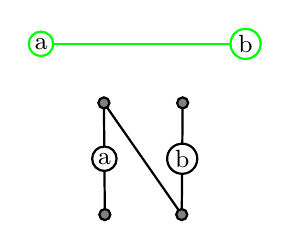
\begin{tikzpicture}[thick,scale=0.5]

	\coordinate (a0) at (0:0);
	\coordinate (a1) at (180:1);
	\coordinate (a3) at (-109:3);
	\coordinate (a2) at (0:1);
	\coordinate (a4) at (-71:3);
	\coordinate (b1) at (150:3);
	\coordinate (b2) at (30:3);

	\draw (a1)-- node[lblvertex] {a}(a3);
	\draw (a2)-- node[lblvertex] {b}(a4);
	\draw (a1)--(a4);
	\draw (b1)[green]--(b2);
	%\draw (a0) node {};	
	\draw (a1) node {};
	\draw (a2) node {};
	\draw (a3) node {};
	\draw (a4) node {};
	\draw (b1) node [lblvertex, draw = green]{a};
	\draw (b2) node [lblvertex, draw = green]{b};
\end{tikzpicture}
}\uncover<7>{\qquad\input{coresp3}}
	\end{center}}

\bframe{Connected matching as a clique problem}{
	Thus, we can rephrase the problem of finding a maximum connected matching in $G$ to the problem of finding a maximum green clique in the proximity coloring induced by $L(G)$.\pause\vskip 0.5 cm
	MCP corresponds to the problem of finding a maximum green clique within a given blue-edge free set of vertices.\pause\vskip 0.5 cm
	\begin{prop}
		Any graph $H$ can be realized as a green graph embedded in a blue-edge free set of vertices in the proximity coloring induced by $L(G)$ for some graph $G$. 
	\end{prop}}
	
\bframe{Connected matching as a clique problem}{	
	The proof of the preceeding proposition consists of a very simple construction.\pause \vskip 0.5 cm
	This proposition immediately yields the promised reduction. \pause
	\begin{corollary}
		MAX CLIQUE has a linear time reduction to MCP.
	\end{corollary}  \pause
	Note that we cannot replace MCP with MCM in the above results.  Not every graph is realizable as the green graph in the proximity coloring induced by a line graph.}

\bframe{An MCP-efficient class}{
	Now suppose that $G$ is a graph with $\alpha(G) = 2$. \pause\vskip 0.5 cm
	It is easy to see that the red graph in the proximity coloring induced by $L(G)$ is triangle free.\pause\vskip 0.5 cm
	If the red graph induced by a particular blue free set in the proximity coloring is bipartite, then the maximum green clique is simply the larger half of the bipartition.\pause\vskip 0.5 cm
	
	}

\bframe{An MCP-efficient class}{
	Hence we have the following proposition \pause
	\begin{prop}
		If the red graph of the proximity coloring induced by a graph $G$ with $\alpha(G) = 2$ is bipartite, then MCP can be found in polynomial time for every matching of $G$.
	\end{prop}\pause\vskip 0.5 cm
	In particular, this includes $G$ perfect with $\alpha(G)= 2$.\pause\vskip 0.5cm
	}

\bframe{Perfect green graphs}{
	More generally, we can solve clique problems efficiently on perfect graphs. \pause\vskip 0.5 cm
	Therefore we have the following theorem
	\begin{theorem}
		MCM is polytime solvable on the class of graphs $G$ for which the proximity coloring induced by $L(G)$ has a perfect green graph.
	\end{theorem}\pause
	This fact warrants further study of proximity colorings as such. \pause\vskip 0.5 cm
	It is hoped that a good characterization of this class can be found.}

\bframe{Thank you}{Questions?}

%\begin{bibsection}[Annotated Bibliography]\vspace{-\parskip} % This is the start of the bibliography. 
%	\begin{biblist}[\normalsize] % Replace the \bib entries with ones relevant to your problem.
							% The bulk of each entry can be copied and pasted from MathSciNet
							% ( http://www.ams.org/mathscinet/ ). When viewing the review of an
							% item you want to site, open the "Select alternative format" pull-down
							% and select AMSrefs.
							% Most likely, the only part you will need to change is the first parameter
							% after \bib. This is the internal name you use to cite the reference
							% with \cite. By default it will be the Mathematical Reviews number
							% (for example MR1375315). To make my life easier when I merge these all
							% into the summary document, please choose a name that begins with your
							% initials, followed by the number of problems you have submitted
							% (including this one).
							% For example, since this problem was submitted by Leonhard Euler and
							% since this is the first problem he is presenting, all citation names
							% begin with "le1". If this was his third problem, they would begin with
							% "le3".
%Z. Füredi, A. Gyárfás, G. Simonyi,  Connected matchings and Hadwiger's conjecture,  Combin. Probab. Comput., Problem Section, 14 (2005), 435--438.
%M. Kriesell, On seymour's strengthening of Hadwidger's conjecture for graphs with certain forbidden subgraphs 

%Mukhopadhyay, A. "The Square Root of a Graph." J. Combin. Th. 2, 290-295, 1967. 
\begin{thebibliography}{10}

\bib{MR671905}{article}{
   author={Duchet, P.},
   author={Meyniel, H.},
   title={On Hadwiger's number and the stability number},
   conference={
      title={Graph theory},
      address={Cambridge},
      date={1981},
   },
   book={
      series={North-Holland Math. Stud.},
      volume={62},
      publisher={North-Holland},
      place={Amsterdam},
   },
   date={1982},
   pages={71--73},
   review={\MR{671905 (84h:05074)}},
}

\bib{MR882610}{article}{
   author={Maffray, F.},
   author={Meyniel, H.},
   title={On a relationship between Hadwiger and stability numbers},
   journal={Discrete Math.},
   volume={64},
   date={1987},
   number={1},
   pages={39--42},
   issn={0012-365X},
   review={\MR{882610 (88g:05076)}},
   doi={10.1016/0012-365X(87)90238-X},
}


\bib{MR1411244}{article}{
   author={Toft, Bjarne},
   title={A survey of Hadwiger's conjecture},
   note={Surveys in graph theory (San Francisco, CA, 1995)},
   journal={Congr. Numer.},
   volume={115},
   date={1996},
   pages={249--283},
   issn={0384-9864},
   review={\MR{1411244 (97i:05048)}},
}
\bib{MR1654153}{article}{
   author={Reed, Bruce},
   author={Seymour, Paul},
   title={Fractional colouring and Hadwiger's conjecture},
   journal={J. Combin. Theory Ser. B},
   volume={74},
   date={1998},
   number={2},
   pages={147--152},
   issn={0095-8956},
   review={\MR{1654153 (99k:05079)}},
   doi={10.1006/jctb.1998.1835},
}
\bib{MR1844036}{article}{
   author={Kotlov, Andre{\u\i}},
   title={Matchings and Hadwiger's conjecture},
   note={Algebraic and topological methods in graph theory (Lake Bled,
   1999)},
   journal={Discrete Math.},
   volume={244},
   date={2002},
   number={1-3},
   pages={241--252},
   issn={0012-365X},
   review={\MR{1844036 (2002k:05087)}},
   doi={10.1016/S0012-365X(01)00087-5},
}



\bib{MR2163948}{article}{
   author={Cameron, Kathie},
   title={Connected matchings},
   conference={
      title={Combinatorial optimization---Eureka, you shrink!},
   },
   book={
      series={Lecture Notes in Comput. Sci.},
      volume={2570},
      publisher={Springer},
      place={Berlin},
   },
   date={2003},
   pages={34--38},
   review={\MR{2163948 (2006c:90072)}},
   %doi={10.1007/3-540-36478-1_5},
}

\bib{MR1979786}{article}{
   author={Klazar, Martin},
   title={Non-$P$-recursiveness of numbers of matchings or linear chord
   diagrams with many crossings},
   note={Formal power series and algebraic combinatorics (Scottsdale, AZ,
   2001)},
   journal={Adv. in Appl. Math.},
   volume={30},
   date={2003},
   number={1-2},
   pages={126--136},
   issn={0196-8858},
   review={\MR{1979786 (2004h:05006)}},
   doi={10.1016/S0196-8858(02)00528-6},
}



\bib{MR2070161}{article}{
   author={Plummer, Michael D.},
   author={Stiebitz, Michael},
   author={Toft, Bjarne},
   title={On a special case of Hadwiger's conjecture},
   journal={Discuss. Math. Graph Theory},
   volume={23},
   date={2003},
   number={2},
   pages={333--363},
   issn={1234-3099},
   review={\MR{2070161 (2005e:05055)}},
}

\bib{FGS}{article}{
   author={F\"{u}redi, Zolt\'{a}n},
   author={Gy{\'a}rf{\'a}s, Andr{\'a}s},
   author={Simonyi, G\'{a}bor}
   title={Connected matchings and Hadwiger's conjecture},
   journal={Combin. Probab. Comput.},
   part={Problem Section},
   volume={14},
   date={2005},
   pages={435--438},
}


\bib{MR2156345}{article}{
   author={Kawarabayashi, Ken-ichi},
   author={Plummer, Michael D.},
   author={Toft, Bjarne},
   title={Improvements of the theorem of Duchet and Meyniel on Hadwiger's
   conjecture},
   journal={J. Combin. Theory Ser. B},
   volume={95},
   date={2005},
   number={1},
   pages={152--167},
   issn={0095-8956},
   review={\MR{2156345 (2006b:05118)}},
   doi={10.1016/j.jctb.2005.04.001},
}


\bib{MR2249267}{article}{
   author={Gy{\'a}rf{\'a}s, Andr{\'a}s},
   author={Ruszink{\'o}, Mikl{\'o}s},
   author={S{\'a}rk{\"o}zy, G{\'a}bor N.},
   author={Szemer{\'e}di, Endre},
   title={One-sided coverings of colored complete bipartite graphs},
   conference={
      title={Topics in discrete mathematics},
   },
   book={
      series={Algorithms Combin.},
      volume={26},
      publisher={Springer},
      place={Berlin},
   },
   date={2006},
   pages={133--144},
   review={\MR{2249267 (2008c:05120)}},
   %doi={10.1007/3-540-33700-8_8},
}

\bib{FGS}{article}{
   author={Kriesell, Matthias},
   title={On Seymour's strengthening of Hadwiger's conjecture for graphs with certain forbidden subgraphs},
   journal={Discrete Mathematics},
   %volume={},
   date={2010},
   pages={435--438},
}

\bib{MR0297600}{article}{
   author={Chv{\'a}tal, V.},
   author={Erd{\H{o}}s, P.},
   title={A note on Hamiltonian circuits},
   journal={Discrete Math.},
   volume={2},
   date={1972},
   pages={111--113},
   issn={0012-365X},
   review={\MR{0297600 (45 \#6654)}},
}

\bib{MR1369063}{article}{
   author={Kim, Jeong Han},
   title={The Ramsey number $R(3,t)$ has order of magnitude $t\sp 2/\log t$},
   journal={Random Structures Algorithms},
   volume={7},
   date={1995},
   number={3},
   pages={173--207},
   issn={1042-9832},
   review={\MR{1369063 (96m:05140)}},
   doi={10.1002/rsa.3240070302},
}

\bib{MR0284366}{article}{
   author={Nash-Williams, C. St. J. A.},
   title={Edge-disjoint Hamiltonian circuits in graphs with vertices of
   large valency},
   conference={
      title={Studies in Pure Mathematics (Presented to Richard Rado)},
   },
   book={
      publisher={Academic Press},
      place={London},
   },
   date={1971},
   pages={157--183},
   review={\MR{0284366 (44 \#1594)}},
}

\bib{edhc}{article}{
	author={Christofides, Demetres},
	author={K\"{u}hn, Daniela},
	author={Osthus, Deryk},
	title={Edge-disjoint Hamilton cycles in graphs},
	date={31 Aug 2009},
	eprint={arXiv:0908.4572v1 [math.CO]},
	url={http://arxiv.org/abs/0908.4572},
}

\bib{MR1851303}{book}{
   author={Vazirani, Vijay V.},
   title={Approximation algorithms},
   publisher={Springer-Verlag},
   place={Berlin},
   date={2001},
   pages={xx+378},
   isbn={3-540-65367-8},
   review={\MR{1851303 (2002h:68001)}},
}

\end{thebibliography}
\nocite{*}
\end{document}
